%!TEX root = ../dynamics.tex
\section{Analyzing the Features Affecting Batch Throughput}
\label{sec:throughput}
Next, we turn our attention to analyzing the factors that influence the  progress (or completion) of a batch, how those factors influence each other and how they evolve over time.

\subsection{A Machine Learning Approach}
In order to conduct this analysis, we model the task of batch throughput prediction as a regression problem.  Some of the  29  features we use for this task are the ones used in the previous section to classify HIT type.  We describe the remaining ones in appendix A. The value  we aim to predict (i.e.,   $DIFF\_HIT$) is the batch \emph{throughput}, that is, the numbers of HITs that   will be completed for a given batch within the next time frame of 1 hour.

\begin{figure}[tb]
	\centering
		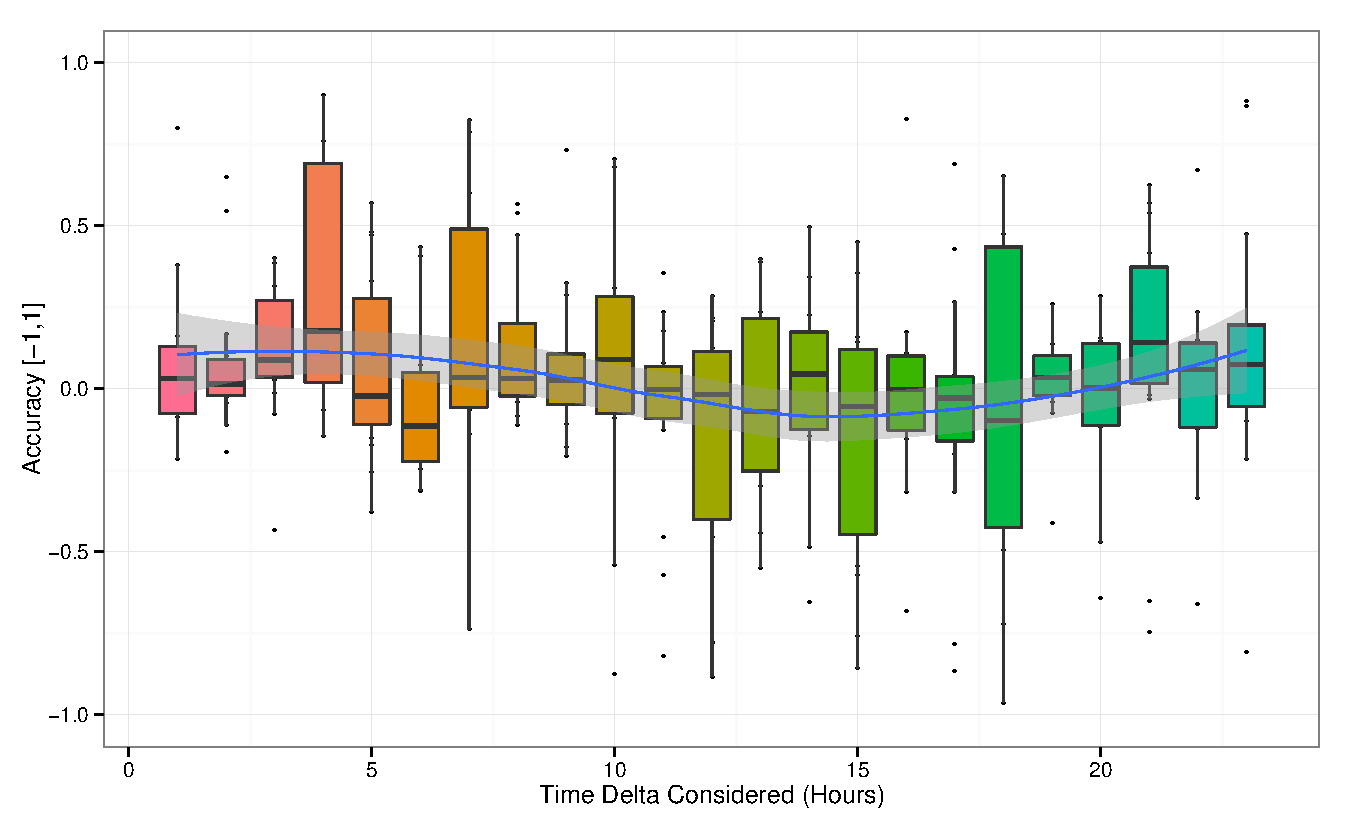
\includegraphics[width=0.48\textwidth]{figures/ML_accuracy}
	\caption{Score ($R^2$) of the throughput prediction when considering larger time spans as training sets. The red dots are average values, while the boxes represents the median, first and third quartiles.}
	\label{fig:accuracy}
\end{figure}

\begin{figure}[tb]
	\centering
		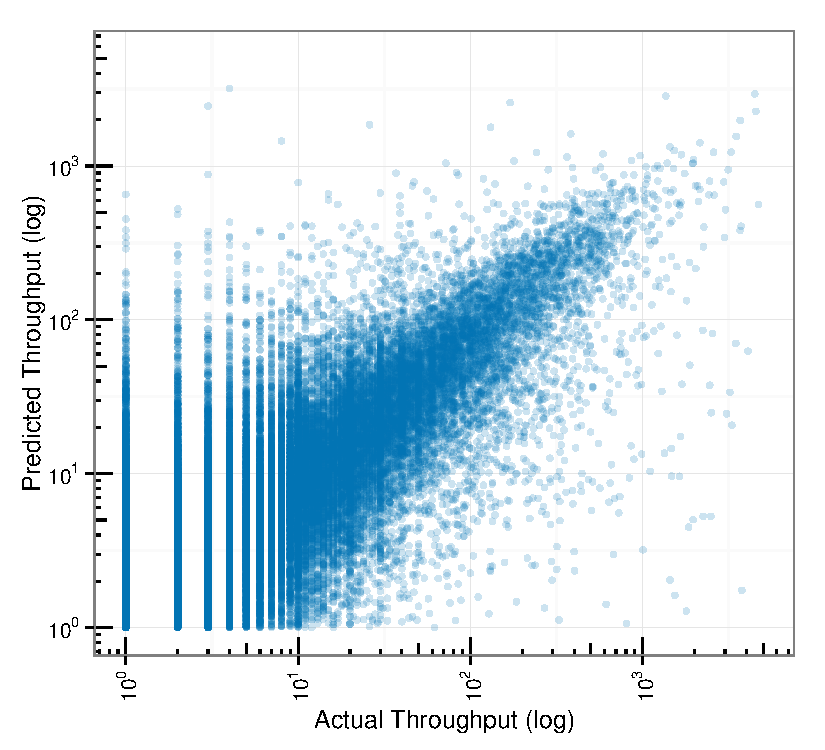
\includegraphics[width=0.48\textwidth]{figures/predictions_3}
	\caption{Prediction vs actual throughput values. Prediction is more accurate for larger throughput values. This suggests that the throughput will remain high until the batch gets smaller.}
	\label{fig:pred}
\end{figure}

In detail, to predict the throughput of a batch at time $T$, we train a Random Forest Regression model with samples taken in the range $[T-\delta, T)$ where $\delta$ is the size of the time window that we are   considering directly prior to time $T$. The rational behind this approach is that the throughput should be directly correlated to the current and recent market situations. 
The research question we tackle in this context is: ``How much historical data dow one need to consider to predict the throughput effectively?". To answer this, we proceed by varying $\delta$.
To evaluate the effectiveness of $\delta$ values, we compute the coefficient of determination  $R^2$ \cite{sklearnweb, sklearn}.
In this experiment, we considered  data from June to October 2014 and hourly observations (see Section \ref{sec:tracker}), from which we uniformly sampled 50 time points for evaluation purposes. Finally, for each time point we considered a training time frame $\delta$ ranging from 1 hour to 24 hours. 

In Figure \ref{fig:accuracy}, we observe that the computed evaluation score reaches its highest values when using the latest 4 hours as training time-frame, then decreases when we increase the training time-frame, to finally again increase and stabilize when we use up to 24 hours training data.
Note that the score is relatively low for batches with low throughput. The prediction works best for larger batches having a large momentum as Figure \ref{fig:pred} suggests.



\begin{figure}[tb]
	\centering
		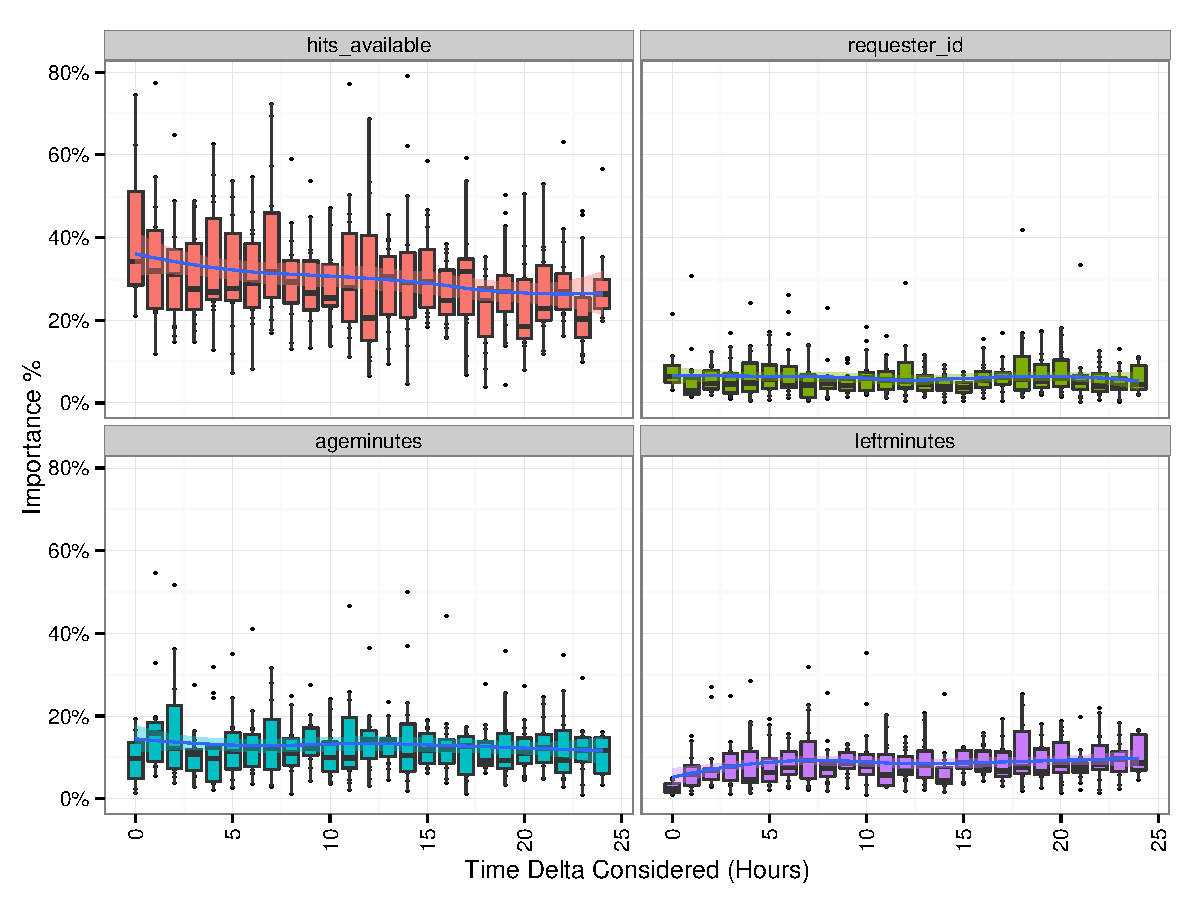
\includegraphics[width=0.5\textwidth]{figures/importances}
	\caption{Computed feature importance when considering larger training sets for the prediction.}
	\label{fig:importances}
\end{figure}


In order to better grasp the characteristics of our throughput prediction, we examine the feature importance. Figure \ref{fig:importances} shows the  contribution of each feature and how it varies  when we increase the training time-frame.
The most important feature is $HIT\_Available$, that is, the current size of the batch. Indeed, as observed by previous work, larger batches tend to attract more workers \cite{mturk,crowddb}. This feature becomes less important when we consider longer periods, partly because of noise, but, most importantly, because of other features like $age\_minutes$ and $left\_minutes$, which encode additional facts and suggest that the crowd is sensitive to the newly posted HITs, or how \emph{fresh} the HITs are. To better understand this phenomenon, we conduct an analysis on what attracts the workforce to the the platform in the next section .

